%!TEX root = paper.tex
% \section{Synthesizing \DIs}

\looseness-1 In this section, we describe our techniques for deriving \dis. We
start with the synthesis of simple \invariants (the $\phi$ \invariants in
our language specification), followed by compound \invariants (the $\Psi$
\invariants in our language specification). Finally, we analyze the time and
memory complexity of our algorithm.

\subsection{Simple \DIs}\label{sec:conjunctive} Synthesizing simple \dis
involves (a)~discovering the \views, and (b)~discovering the lower and upper
bounds for each \view. We start by discussing~(b), followed by the principle to
identify effective \views, based on which we solve~(a).


\subsubsection{Synthesizing Bounds for \Views}\label{synth-bounds} Fix a \view $F$
and consider the bounded-\view \invariant $\phi$: $\lb \leq
F(\vec{A}) \leq \ub$. 
% Now, the tightest bounds for this form, for a dataset $D$,
% is given by $\ub = \max(F(D))$ and $\lb = \min(F(D))$.
% However, this choice is very sensitive to noise:
% adding a single ``atypical'' tuple to $D$ can produce very different
% \invariants.
Given a dataset $D$, a trivial choice for the bounds
% valid on all tuples in a dataset $D$ 
is: $\lb = \min(F(D))$ and $\ub = \max(F(D))$. However, this choice is very
sensitive to noise: adding a single atypical tuple to $D$ can produce very
different \invariants.
% To concretize the \invariant, we need to instantiate
% the \view $F$, and the bounds $\lb$ and $\ub$.
% We provide a constructive
% mechanism to synthesize \views for linear \invariants in
% Section~\ref{sec:pca-invs}. Here, we focus on the constants $\lb$ and $\ub$.
% For a \view $F$, we compute $\lb$ and $\ub$ as follows:
%
% However, it suffers from two issues: (1)~if $F(D)$ has very low variance (e.g.,
% a constant), then the \invariant may become too tight, and (2)~if there is even
% a single atypical tuple in $D$, the bound can be too loose.
% However, it suffers from two issues: (1)~if $F(D)$ has very low variance (e.g.,
% a constant), then the \invariant may become too tight, and (2)~if there is even
% a single atypical tuple in $D$, the bound can be too loose.
Instead, we use a more robust choice as follows:
%, at the cost of potentially having a small number of tuples in $D$ that do not satisfy the \invariant:
%
\begin{align*}
    \lb = \avg{F(D)} - C \cdot \stddev{F(D)}, \;\;\;\;
    \ub = \avg{F(D)} + C \cdot \stddev{F(D)}
\end{align*}
%
\looseness-1
Here, $\avg{F(D)}$ and $\stddev{F(D)}$ denote the mean and standard deviation
of the values in $F(D)$, respectively, and $C$ is some positive constant.
With these bounds, $\semq{\phi}(t) = 0$ implies that
%\begin{enumerate*}[label=(\alph*)]
    %\item 
        $F(t)$ is within $C \times \stddev{F(D)}$ from the mean $\avg{F(D)}$. % \emph{and}
    %\item $F(t)$ is between $\min(F(D))$ and $\max(F(D))$.
%\end{enumerate*}
%
%
%
%Consequently, some 
% Since there can be tuples $t\in D$ that are more than $C$ standard
% deviations away from the mean,
% % These tuples are considered outliers, and
% $\phi$ is a \invariant for the subset of $D$ that excludes some ``outliers'';
% this is often desirable for many practical applications.
% that are more then $4$ standard
% deviations away from the mean may violate $\phi$; so, $\phi$ may not be an
% \invariant for $D$, but only for some subset of $D$ that does not contain any
% outlier. 
% However, this is often desirable for many practical applications.
%
In our experiments, we set $C = 4$, which ensures that in expectation, very few
tuples in $D$ will violate the \invariant for many distributions of the values
in $F(D)$. Specifically, if $F(D)$ follows a normal distribution, then
$99.99\%$ of the population is expected to lie within $4$ standard deviations
from mean. \reviseone{Note that we make no assumption on the original data
distribution of each attribute.}


% Since a-priori we have no knowledge of the underlying distribution of the
% values in $F(D)$, we assume that the distribution is normal and therefore, we
% use $C = 4$ in our experiments.\footnote{\scriptsize{For normal distributions,
% $99.99\%$ of the population is expected to lie within $4$ standard deviations
% from mean. Only 1 in 15787 tuples falls outside this range.}}

%Note that the choice of $\lb$ and $\ub$ is not restricted to the above and one
%can follow a different design choice for computing the bounds, guided by the
%assumption of distribution of $F(D)$ in associated application.
% the quantitative semantics of data
% \invariant is not limited to this assumption and can support assumption of any
% distribution, given a procedure to compute $\lb$ and $\ub$ is available.}
%
%
% \smallskip
%
Setting the bounds $\lb$ and $\ub$ as $C\cdot\stddev{F(D)}$-away from the mean,
and the scaling factor $\alpha$ as $\frac{1}{\stddev{F(D)}}$, guarantees the
following property for our quantitative semantics:
% As long as the scaling factor $\alpha=\frac{1}{\stddev{F(D)}}$ and
% the bounds $\lb,\ub$ are given by $\avg{F(D)}\pm C*\stddev{F(D)}$ for some $C$,
% %However, regardless of the choice of bounds $\lb$ and $\ub$,
% the quantitative semantics has the following nice property.
%
\begin{figure}
	\centering
	\resizebox{0.8\columnwidth}{!}{
	\begin{subfigure}{.18\textwidth}
	  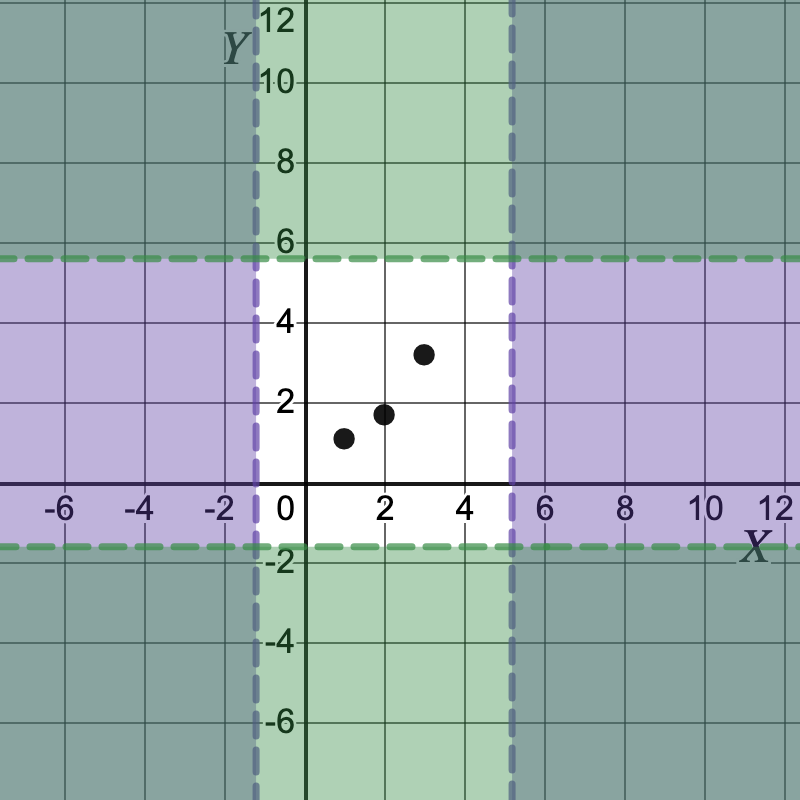
\includegraphics[width=1\linewidth]{Figures/view1.png}
	  \vspace{-6mm}
	  \caption{}
	  \label{subfig:views1}
	\end{subfigure}%
	\hspace{5mm}
	\begin{subfigure}{.18\textwidth}
	  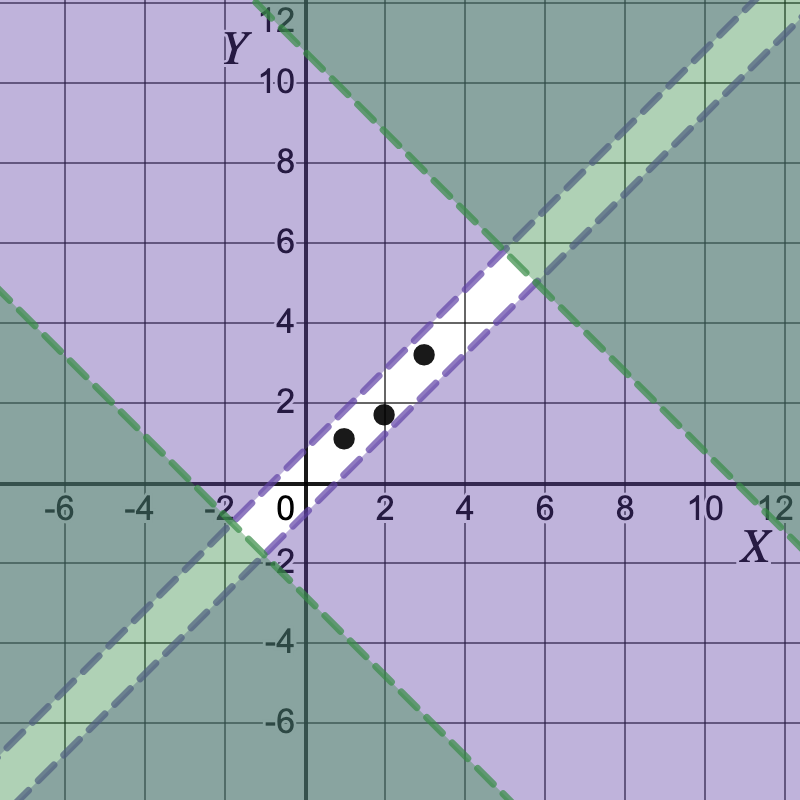
\includegraphics[width=1\linewidth]{Figures/view2.png}
	  \vspace{-6mm}
	  \caption{}
	  \label{subfig:views3}
	\end{subfigure}
	}
	\vspace{-4mm}
        \caption{\small
		\looseness-1
		Clear and shaded regions depict conformance and non-conformance zones, respectively.
		(a)~Correlated projections $X$ and $Y$ yield \dis forming a large conformance zone, % resulting in an underfitted data profile.
		(b)~Uncorrelated (orthogonal) projections $X-Y$ and $X+Y$ yield \dis forming a smaller conformance zone.%, resulting in an optimal data profile.
		}
	\label{fig:views}
	\vspace{-3mm}
\end{figure}

\begin{lemma}\label{lemma:helper}
    Let $D$ be a dataset and let 
    $\phi_k$ be $\lb_k \leq F_k(\vec{A})\leq \ub_k$ for $k=1,2$.
    Then, for any tuple $t$, if 
    $\frac{|F_1(t) - \avg{F_1(D)}|}{\stddev{F_1(D)}} \geq \frac{|F_2(t) - \avg{F_2(D)}|}{\stddev{F_2(D)}}$,
    then $\semq{\phi_1}(t) \geq \semq{\phi_2}(t)$.
\end{lemma}
%
This means that larger deviation from the mean (proportionally to
the standard deviation) results in higher degree of violation under our
semantics. The proof follows from the fact that the normalization function
$\eta(.)$ is monotonically increasing, and hence, $\semq{\phi_k}(t)$ is a
monotonically non-decreasing function of $\frac{|F_k(t) -
\avg{F_k(D)}|}{\stddev{F_k(D)}}$.


\subsubsection{Principle for Synthesizing \Views}\label{view-synthesis}
%
% \looseness-1
% One question naturally arises: what \views should we use to synthesize
% \invariants for $D$? Does it even matter what \views we pick, or would any choice
% be equally effective? To answer these questions, we need to first understand
% what makes a \invariant more effective than others for a particular task. For
% many practical applications, \invariants of \emph{moderate} strength are most
% effective. Ideally, we look for two criteria in an effective \invariant: (1)~it
% should not overfit the data, rather should generalize by capturing the
% properties of the data, (2)~it should not underfit the data, because majority
% of the tuples within the data domain would then satisfy such \invariant. To
% satisfy the first criterion, we allow flexible bounds---specified using $\lb$
% and $\ub$---as discussed earlier. To satisfy the second criterion, we
% pick \views that produce strong \invariants.
% %among a set of possible \invariants, with
% %respect to a large subset of the data domain.

\looseness-1 %To understand how to derive the \views for effective \dis, 
We start by investigating what makes a \invariant more effective than others.
An effective \invariant (1)~should not overfit the data, but rather generalize
by capturing the properties of the data, and (2)~should not underfit the data,
because it would be too permissive and fail to identify deviations effectively.
Our flexible bounds (Section~\ref{synth-bounds}) serve to avoid overfitting. In
this section, we focus on identifying the principles that help us avoid
underfitting. We first describe the key technical ideas for characterizing
effective \views through example and then proceed to formalization.

% https://www.desmos.com/calculator/zrtfddd6dn
% 
\begin{example}\label{ex:badproj}
	%
	 \looseness-1 Let $D$ be a dataset of three tuples
	 \{(1,1.1),(2,1.7),(3,3.2)\} with two attributes $X$ and $Y$. Consider two
	 arbitrary \views: $X$ and $Y$. For $X$: $\mu(X(D)) = 2$ and $\sigma(X(D)) =
	 0.8$. So, bounds for its \di are: $\lb = 2 - 4 \times 0.8 = -1.2$ and $\ub =
	 2 + 4 \times 0.8 = 5.2$. This gives us the \di: $-1.2 \le X \le 5.2$.
	 Similarly, for $Y$, we get the \di: $-1.6 \le Y \le 5.6$.
	 Fig.~\ref{subfig:views1} shows the conformance zone (clear region) defined by
	 these two \dis. The shaded region depicts non-conformance zone. The
	 conformance zone is large and too permissive: it allows many atypical tuples
	 with respect to $D$, such as $(0,4)$ and $(4, 0)$.
	%
\end{example}

A natural question arises: are there other \views that can better characterize
conformance with respect to the tuples in $D$? The answer is yes and next we
show another pair of \views that shrink the conformance zone significantly.

\begin{example}\label{ex:goodproj} 
	%
	 In Fig.~\ref{subfig:views3}, the clear region is defined by the \dis $-0.8
	 \le X - Y \le 0.8$ and $-2.8 \le X + Y \le 10.8$, over \views $X-Y$ and
	 $X+Y$, respectively. The region is indeed much smaller than the one in
	 Fig.~\ref{subfig:views1} and allows fewer atypical tuples.
	 %
\end{example}




How can we derive \view $X-Y$ from the \views $X$ and $Y$, given $D$? Note that
$X$ and $Y$ are highly correlated in $D$. In Lemma~\ref{LEMMA:MAIN}, we show
that two highly correlated \views can be linearly combined to construct another
\view with lower standard deviation that generates a \emph{stronger} \invariant.
%We later generalize this result to
%multiple \views in Theorem~\ref{THM:MAIN}. 
We proceed to formalize {\em{stronger \invariant}}---which defines whether a
\invariant is more effective than another in quantifying violation---and
\emph{incongruous tuples}---which help us estimate the subset of the data
domain for which a \invariant is stronger than the others.

\begin{definition}[Stronger \invariant]\label{def:stronger}
	\begin{sloppypar}
A \di $\phi_1$ is stronger
than another \di $\phi_2$ on a subset $H \subseteq \DDom^m$ if
$\forall t \in H, \; \semq{\phi_1}(t) \geq \semq{\phi_2}(t)$.
	\end{sloppypar}
\end{definition}

%
Given a dataset $D\subseteq \DDom^m$ and a \view $F$, for any tuple $t$, let
$\delF{F}{t} = F(t) - \avg{F(D)}$. For \views $F_1$ and $F_2$, the correlation
coefficient $\rho_{F_1,F_2}$ (over $D$) is defined as
$\frac{\frac{1}{|D|}\sum_{t\in D}
\delF{F_1}{t}\delF{F_2}{t}}{\stddev{F_1(D)}\stddev{F_2(D)}}$.
%
\begin{definition}[Incongruous tuple]	
A tuple $t$ is {\em{incongruous}} w.r.t.\ a
\view pair $\!\langle F_1, F_2\rangle\!$ on $D$ if: 
$\delF{F_1}{t}\cdot\delF{F_2}{t}\cdot\rho_{F_1,F_2}<0$.
%
\end{definition}



Informally, an incongruous tuple for a pair of \views does not follow the
general trend of correlation between the \view pair. For example, if $F_1$ and
$F_2$ are positively correlated ($\rho_{F_1,F_2}>0$), an incongruous tuple $t$
deviates in opposite ways from the mean of each \view
($\delF{F_1}{t}\cdot\delF{F_2}{t}<0$). Our goal is to find \views that yield a
conformance zone with very few incongruous tuples.

\begin{example} 
	%
	In Example~\ref{ex:badproj}, $X$ and $Y$ are positively
correlated with $\rho_{X,Y} \approx 1$. The tuple
$t=(0,4)$ is incongruous w.r.t. $\langle X, Y \rangle$, because $X(t) = 0 <
\mu(X(D)) = 2$, whereas $Y(t) = 4 > \mu(Y(D)) = 2$. Intuitively, the
incongruous tuples do not behave like the tuples in $D$ when viewed through the
\views $X$ and $Y$. Note that the narrow conformance zone of
Fig.~\ref{subfig:views3} no longer contains the incongruous tuple $(0, 4)$.
In fact, the conformance zone defined by the \dis derived from \views $X - Y$
and $X + Y$ are free from a vast majority of the incongruous tuples.
%
\end{example}


We proceed to state Lemma~\ref{LEMMA:MAIN}, which informally says that any two
highly correlated \views can be linearly combined to construct a new \view to
obtain a stronger \invariant. We write $\phi_F$ to denote the \di $\lb \le
F(\vec{A}) \le \ub$, synthesized from $F$. (All proofs are in \appOrTechRep.)



\begin{lemma}\label{LEMMA:MAIN}
    Let $D$ be a dataset and $F_1,F_2$ be two \views on $D$ s.t.\ $|\rho_{F_1,F_2}| \geq \frac{1}{2}$.
    Then, $\exists \beta_1, \beta_2 \in \Real$ s.t.\ $\beta_1^2 + \beta_2^2 = 1$ and for the new \view
    $F = \beta_1 F_1 + \beta_2 F_2$:
	 %
	 \begin{enumerate}[label=(\arabic*)]
	     \item $\stddev{F(D)} < \stddev{F_1(D)}$ and $\stddev{F(D)} < \stddev{F_2(D)}$, and
         \item $\phi_F$ is stronger than both $\phi_{F_1}$ and $\phi_{F_2}$
     on the set of tuples that are incongruous w.r.t. $\!\langle F_1,
     F_2\rangle$.
	 \end{enumerate} 
	 %
% Here $\phi_F$ just denotes $\lb \leq F(\vec{A}) \leq \ub$,
%      where $\lb,\ub$ are as defined above.
	 %
    %$\mathtt{sign}((F_1(t) - \avg{F_1(D)}) * (F_2(t) - \avg{F_2(D)}) * \rho_{F_1(D),F_2(D)}) = -1$,
\end{lemma}
%

\noindent We now extend the result to multiple \views in Theorem~\ref{THM:MAIN}.
%

\begin{theorem}[Low Standard Deviation \Invariants]\label{THM:MAIN}
	%\sloppy
    Given a dataset $D$, let $\mathcal{F} {=} \{F_1,\ldots,F_K\}$ denote a set of \views on $D$
    s.t.\ $\exists F_i,F_j{ \in }\mathcal{F}$ with $|\rho_{F_i,F_j}| {\geq} \frac{1}{2}$.
    Then, there exist a nonempty subset $I {\subseteq} \{1,\ldots,K\}$ and a \view
    $F {=} \sum_{k\in I} \beta_k F_k$, where $\beta_k {\in} \Real$ s.t.
    \begin{enumerate}[label=(\arabic*)]
        \item $\forall k\in I$, $\stddev{F(D)} < \stddev{F_k(D)}$,
        \item $\forall k\in I$, $\phi_F$ is stronger than $\phi_{F_k}$ on the subset $H$, where\\ 
	$H {=} \{t \mid 
		\forall {k{\in} I} (\beta_k \delF{F_k}{t} {\geq} 0) \vee 
		\forall {k{\in} I} (\beta_k \delF{F_k}{t} {\leq} 0)\}$, and
        \item $\forall k\not\in I$, $|\rho_{F,F_k}| < \frac{1}{2}$.
    \end{enumerate}
    %     (1)~$\stddev{F(D)} < \stddev{F_k(D)}$ for all $k\in I$, and
    %     \\
    %     (2)~$\phi_F$ is stronger than $\phi_{F_k}$
    %     % $\semq{\phi_F}(t) \geq \semq{\phi_{F_k}}(t)$ for each $i$ and
    %     on the subset $H$ of tuples,
    %     where
    % $H = \{t \mid
    %     (\bigwedge_{k\in I}\beta_k \delF{F_k}{t} \geq 0) \vee
    %     (\bigwedge_{k\in I}\beta_k \delF{F_k}{t} \leq 0)\}$.
\end{theorem}



\looseness-1 The theorem establishes that to detect violations for tuples
in~$H$: (1)~\views with low standard deviations define stronger \invariants
(and, thus, are preferable), and (2)~a set of \invariants with highly correlated
\views is suboptimal (as they can be linearly combined to generate stronger
\invariants).
% 
% The tuples in $H$ disagree with the mutual
% correlation between attributes, whereas the tuples not in $H$ have at least some (partial) agreement
% with these correlations.  
%
%The application determines if it is important to put more emphasis on the
%tuples in $H$ than the tuples in the complement of $H$. 
Note that $H$ is a conservative estimate for the set of tuples where $\phi_F$
is stronger than each $\phi_{F_k}$; there exist tuples outside $H$ for which
$\phi_F$ is stronger.

\revisethree{ 
%
\smallskip

\paragraph{Bounded \views vs.\ convex polytope.} \label{polytope} Bounded
projections (Example~\ref{ex:goodproj}) relate to the computation of convex
polytopes~\cite{turchini2017convex}. For example, one can compute a convex
hull---the minimal convex polytope that includes all the training tuples---and
then any tuple falling outside it is considered non-conforming. However, a
convex hull overfits to the training tuples and is extremely sensitive to
outliers. For example, consider a training dataset over attributes $X$ and $Y$:
$\{(1, 10), (2,20), (3, 30)\}$. A convex hull in this case would be a line
segment---starting at $(1, 10)$ and ending at $(3, 30)$---and the tuple $(5,
50)$ will fall outside it.
%
%
% Instead of a
% set of bounded \views, as shown in Example~\ref{ex:goodproj}, an alternative
% approach is to compute a convex polytope~\cite{turchini2017convex}---the
% smallest possible convex set of tuples that includes all the training tuples;
% then any tuple falling outside the polytope is marked as non-conforming.
% However, such an approach tends to overfit the training tuples and is extremely
% sensitive to outliers. For example, consider a training dataset over attributes
% $X$ and $Y$: $\{(1, 10), (2,20), (3, 30)\}$. A convex polytope in this case
% would be a line segment---starting at $(1, 10)$ and ending at $(3, 30)$---and
% the tuple $(5, 50)$ will fall outside it.
%
Unlike convex hull---whose goal is to find the smallest possible
``inclusion zone'' that includes all training tuples---our goal is to find a
``conformance zone'' that reflects the \emph{trend} of the training tuples.
This is inspired from the fact that ML models aim to generalize to tuples
outside training set; thus, \dis also need to capture trends and avoid
overfitting. Our definition of good \dis (low variance and low mutual
correlation) balances overfitting and overgeneralization. Therefore, beyond the
minimal bounding hyper-box over the training tuples, we take into consideration
the distribution of the \emph{interaction} among attributes (trends). For the
above example, \dis will model the interaction trend: $Y = 10X$, allowing the
tuple $(5, 50)$.
%, which follows the same trend as the training tuples.
%
}


\ignore{
\begin{example}%[Low standard deviation \views]
	\label{ex:lowvar}
	%\looseness-1	
	%
    Consider $D = \{(1,1), (2,2), (3,3)\}$ and \views $F_1(A_1,A_2) =
    A_1$ and $F_2(A_1,A_2) = A_2$. On $D$, both \views have the same mean
    $\avg{F_1(D)} = \avg{F_2(D)} = 2$ and standard deviation 
    $\stddev{F_1(D)} = \stddev{F_2(D)} = \sqrt{2/3}$.
	%
	% that is,
	%     $$
	%     \stddev{F_1(D)} = \stddev{F_2(D)} = 
	%	\sqrt{\frac{(1{-}2)^2{+}(2{-}2)^2{+}(3{-}2)^2}{3}} = \sqrt{\frac{2}{3}}
	%     $$
	% \af{check std value. It was 1 before, but that was incorrect. I corrected it to be $\sqrt{2/3}$}
	%
    The correlation coefficient is $\rho_{F_1,F_2} = 1$ since $F_1 = F_2$
    on $D$. 
    We derive a new \view $F = F_1 - F_2$, and note that $F(D) = \{0,0,0\}$ and
    hence, $\stddev{F(D)} = 0 < \sqrt{2/3}$. Furthermore, $\phi_F$ is stronger than
    $\phi_{F_1}$ and $\phi_{F_2}$ on all tuples $t$ s.t.\ $\delF{F_1}{t}\delF{F_2}{t}<0$, i.e., $H = \{t \mid
    (t.{A_1} {>} 2 \wedge t.{A_2} {<} 2) \vee (t.{A_1} {<} 2 \wedge t.{A_2} {>} 2)\}$.
	
    Note that there can be tuples outside of $H$ for which $\phi_F$ is
    not stronger than $\phi_{F_1}$ and $\phi_{F_2}$. For example, for the tuple
    $t = (10,10)$, $F(t) = 0$ and $\delF{F}{t} = 0$. Hence, the \invariant
    $-4\cdot\stddev{F(D)} \leq F(t) \leq 4\cdot\stddev{F(D)}$ is satisfied
    (violation score is $0$). However, the \invariants $-4\cdot\stddev{F_1(D)}
    \leq F_1(t) \leq 4\cdot\stddev{F_1(D)}$ and $-4\cdot\stddev{F_2(D)} \leq
    F_2(t) \leq 4\cdot\stddev{F_2(D)}$ are not satisfied (violation score
    $>0$). The intuition is that $t$ falls outside the observed trends for $F_1$ and 
	$F_2$ ($A_1$ and $A_2$), but it is still within the combined trend ($A_1=A_2$), 
	which better generalized the observed data in $D$.
\end{example}
\endignore}

\ignore{ %% 
%
\begin{remark}[Linear, nonlinear, and differential forms]
%
%
The linear functions $F$ are just linear functionals \af{I don't know what
functionals or one forms are. Can we put a footnote here explaining these two
terms?} (also called one forms) when $\DDom^m$ is \viewed as $n$-dimensional
vector space. Note that $D$ will be \viewed as tuples from some subspace of
dimension $n' \leq n$. It is fairly common for $D$ to lie in lower-dimensional
manifold, and hence $n' < n$. When we do not consider noise in data, equality
\invariants are just annihilators of $D$. So, ideally, we will have $n-n'$
independent \invariants. If the columns represent some continuously changing
quantities, we could consider differential one-forms (as in differential
geometry) as potential \invariants~\cite{Vidyasagar}, which is outside the scope
of this paper. In general, we could also consider nonlinear $F$, for example,
we can get such \invariants from autoencoders.
%
\end{remark}
\endignore}

\def\eig{{\mathcal{E}}}	
\def \categorical {low-cardinality}

\ignore{
In this section, we present an approach for synthesizing compound linear
\invariants, which are \invariants that only use linear \views. We first describe
our approach for generating linear \invariants, and then proceed to describe the
procedure for generating compound \invariants.

\looseness-1
The restriction to linear \views is reasonable because linear relationships
between attributes, whenever they exist, are exploited (as a precondition) to
perform dimensionality reduction in several ML techniques, and thus, they are
{\em{relevant}} to a large class of ML models.

\endignore}

\ignore{

We argued in Section~\ref{sec:di-for-tml} that the choice of the form of
\invariants should be guided by the class of machine learning models. In this
paper, we focus on computing simple \invariants as they are likely to be
relevant for most practical classes of models. To that end, in this section, we
describe the computation of compound linear \invariants using an approach
inspired by principal component analysis (PCA).

Heretofore, we were considering the noise-free scenario where data is assumed
to be perfect, and the intent was to learn models such that their predictions
exactly match the provided labels. Since we want to develop \invariant-learning
procedures that can be evaluated on real-world noisy datasets, henceforth, we
drop this assumption.

In this paper, we restrict ourselves to linear $F$ because linear relationships
between attributes, if they exist, are assumed (as a precondition) to perform
dimensionality reduction in several ML techniques.

We now describe our procedure for synthesizing \dis for a given
dataset. We start by describing \emph{transformations}---which prepares the
dataset for \invariant learning. Then we describe \emph{\atomic\ formulas},
which we use to encode \invariants such that we can quantify violation of the
learned \invariants by a data point. Finally, we describe the PCA-based procedure
for learning linear \invariants which we express using \atomic\ formulas.

\endignore}

\ignore{
\subsection{Transformations} 
A transformation $T$ is a preprocessing step that prepares the dataset $D$ for the \invariant learning procedure.
Some example of transformations include:
(a)~introducing new derived attributes in $D$,
(b)~removing columns from $D$ that should not be part of the learned \invariant,
(c)~reorganizing data in $D$ to reshape it in a form more appropriate for learning \invariants.

In this paper, the only transformations we use are those that remove columns.
For a dataset $D$, that contains non-numerical columns, we remove the
non-numerical columns of $D$ as a preprocessing step, before using the
PCA-based procedure for learning linear \invariants from it.

Our general methodology for constructing \dis is a two step
procedure:
(1)~apply some transformation $T$ on the dataset $D$ to get a new dataset $T(D)$, and
(2)~learn \dis for $T(D)$.
When testing a new dataset $D'$ against a learned \invariant $\phi$, we again
follow two steps: 
(1)~apply the same transformation $T$ on $D'$ to obtain $T(D')$, and 
(2)~evaluate $\phi$ on the transformed dataset to compute the violation, 
$\phi(T(D'))$.

\endignore}

